\documentclass[a4paper, 12pt]{report}
\usepackage[utf8]{inputenc}
\usepackage[swedish,british]{babel}
\usepackage{graphicx}
\usepackage{fancyhdr}

\usepackage{listings}
\usepackage{glossaries}
\pagestyle{fancy}
\begin{document}

\graphicspath{{./images/}}
\title{Smarter and simple Scrabble strategy}
\date{Course: DD143X \\ Supervisor: Johan Boye \\ Kungliga Tekniska Högskolan \\ CSC \\ March 7, 2012}
\author{Frej Connolly \\ Götgatan 78 13TR LÄG1302 \\ 118 30 Stockholm \\ SWEDEN \\ +46(0)73-963 41 90 \\ connolly@kth.se \\
        \and Diana Gren \\ Sköldgatan 8 2TR \\ 118 63 Stockholm \\ SWEDEN \\ +46(0)70-467 47 20 \\ dianagr@kth.se}

\maketitle
\begin{abstract}
The abstract goes here. TODO
\end{abstract}

\selectlanguage{swedish}
\begin{abstract}
Sammanfattning på svenska hamnar här. TODO
\end{abstract}
\selectlanguage{british}
\tableofcontents





\chapter{Introduction}
Scrabble is an old classic game that is fairly easy to learn. However, it is extremely difficult to be a great player. Compared to other classic board games, such as chess, there are more factors to take into consideration when making a move in Scrabble. 

Apart from anagramming and generating words, there are other crucial decisions to make. A player would probably find several legal moves in one round, and then would have to decide which one to place. Choosing the move that generates the highest score is not always the ideal way to go. It could be that making such a move would create a situation in the next round where nothing could be done, or let the opponent score high.

Making the choice of which move to use include many factors, and there are several different techniques and strategies one can follow to make the decision easier. Picking up the bonus squares can generate an extremely high score, hence one strategy is to try to always pick up the bonus squares and prevent the opponent from doing the same. Another way of being successful is to prioritize using letters with high score, since they would not only generate a high total score to the player, but could also create difficult situations in the future if not used as soon as possible.

There are several more possible strategies one can follow, and this study aims to investigate a three of them trying to establish which one is the more rewarding.

\section{Problem statement}
Scrabble requires the players to have a good vocabulary and to become a successful player, some knowledge about how many tiles of each letter is available is preferable. 

When playing, the ability to keep a good balance between consonants and vowels on the rack can profit future moves. Destroying bonus possibilities for the opponent, and at the same time score them oneself is a crucial skill, and experts are probably aware of which tiles have been placed, and those that remain, allowing them to anticipate the future sequence of events. 

\subsection{Question}
Which of the strategies has the most impact on a game? How do the strategies perform against each other, and which one is the most successful one? 


\section {Terminology}
\label{sec:terminology}

\begin{description}
\item{\emph{Anchor square}}: Vacant board square adjacent to a placed tile.

\item{\emph{Bag}} Tiles that have not been drawn by players.

\item{\emph{BOR}}: Balance on rack player.

\item{\emph{BS}}: Bonus square player.

\item{\emph{Cross check set}}: Set of possible letters on an anchor square with regard to adjacent word going vertical from named square.

\item{\emph{DAWG}}: Directed acyclic word graph.

\item{\emph{HSW}}: High score word player.

\item{\emph{Rack}} Tiles on a player's hand. 

\end{description}







\chapter{Background}

\section{Scrabble game rules}
Scrabble is word game were two to four players are given a set of letter tiles to form words to be placed out on a four-cornered board of squares \cite{ABSP} \cite{NASPA} \cite{forbund}.

\begin{figure}[h]
\centering
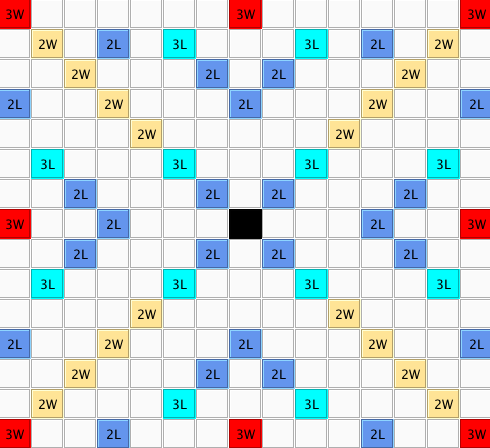
\includegraphics[scale=0.5]{board}
\caption {Game board. 15x15 square board with bonus squares.}
\label{fig:game-board}
\end{figure}

\subsubsection{Game components}
Scrabble consists of 

\begin{itemize}
\item a 15x15 board with bonus squares and the center marked out. fig. \ref{fig:game-board}.
\item a set of letter tiles
\end{itemize}

The players are given 5-8 tiles each to keep on their \emph{rack}. Each letter reward points. Common letters gives lower points. The following list shows letter points and the number of occurances of each tile in the bag. TODO lägg in referens till poänglistan.

\begin{itemize}
\label{letter+table}
	\item{\emph{1 point}} \textbf{A}x8, \textbf{D}x5, \textbf{E}x7, \textbf{I}x5, \textbf{L}x5, \textbf{N}x6, \textbf{R}x8, \textbf{S}x8, \textbf{T}x8
	\item{\emph{2 points}} \textbf{G}x3, \textbf{H}x2, \textbf{K}x3, \textbf{M}x3, \textbf{O}x5
	\item{\emph{3 points}} \textbf{F}x2, \textbf{V}x2, \textbf{Å}x2
	\item{\emph{4 points}} \textbf{B}x2, \textbf{P}x2, \textbf{U}x3, \textbf{Ä}x2, \textbf{Ö}x2
	\item{\emph{7 points}} \textbf{J}x1, \textbf{Y}x1
	\item{\emph{8 points}} \textbf{C}x1, \textbf{X}x1
	\item{\emph{10 points}} \textbf{Z}x1
\end{itemize}

\subsubsection{Objectives}
Each round the player has to construct a word consisting of at least two letters by using the tiles on the rack and the board. Words can be placed horizontally or vertically. Each word layed down has to contain at least one tile from the board. The player starting has to position the first word so one of the letters is on top of the center square.

\subsubsection{Turn}
A player can choose to do one of the following each turn.
\begin{itemize}
\item Lay out a word onto the board. Then pick up new tiles from the bag, so that the player will have a total of 5-8 tiles again (depending on which rule used for tiles on rack).
\item Pass, receiving 0 points.
\item Exchange a number of tiles from the rack with the bag.
\end{itemize}

\subsubsection{Bonus squares}
There are four different types of \emph{bonus squares} dispersed throughout the board. The following bonus types can be used.

\begin{description}
\item{2L:} Double letter
\item{3L:} Triple letter
\item{2W:} Double word
\item{3W:} Triple word
\end{description}

When a tile is placed on top of one of them the player is rewarded a bonus score for either that particular tile or the whole word. Letter bonus is calculated by multiplying the point for the corresponding letter on top of the bonus square by either two or three. Word bonus is multiplied by two or three to the total score of the word. If a tile on a word bonus square is part of both a horizontal and vertical word, the bonus is then applied to both of them respectively. If a word is positioned on top of both letter- and a bonus tiles, the score of the letter bonuses is calculated first before multiplying the word. Bonuses can only be used once when a tile is placed on the square.

If a player has used all the tiles from the rack an additional 50 points is rewarded the player, added after any eventual bonus score.

\subsubsection{Game over}
The game can end in two ways. Either when a player has emptied the rack, and there are no tiles left in the bag. Or when there has been a total number of four moves with zero points in a row, i.e. the players passed or exchanged tiles.

After the game, all the players still having tiles left on the rack will get a score penalty. The sum of the letter points on the rack is removed from the total score. The winner of the game is the player with the highest score after penalty subtractions. 

\section{Research}
This paper will mostly refer to Appel and Jacobsen \cite{fastest} who discovered a way to represent the dictionary wo that it takes up minimum space in memory and an efficient algorithm to find all legal word to place down depending on the tiles on rack and on the board. 

TODO skriv om följande och förklara varför vi inte valde dem 
Sheppard, B., 2002, Towards Perfect Play of Scrabble, Maastricht. \cite{perfectgame}
Gordon, S. A., 1993, A Faster Scrabble Move Generation Algorithm, Software - Practice and experience, Vol. 24(2), 219-232, February 1994. \cite{faster}
Russell S., Norvig P. Artificial Intelligence: A Modern Approach 3rd ed. Prentice Hall. 2009 \cite{ai}
Manning C. D., Raghavan P., Schütze H., Introduction to Information Retrieval, Cambridge University Press, 2008, p. 49-65. \cite{inforetrieve}

\subsection{Dictionary representation}
\label{dic-rep}
Words from a dictionary can be stored by representing the letters as edges in a trie. A path represent a word. Each path can have sub paths that represent shorter word variations by letting the nodes mark the end of a word. Figure \ref{fig:trie}. 

\begin{figure}[h]
\centering
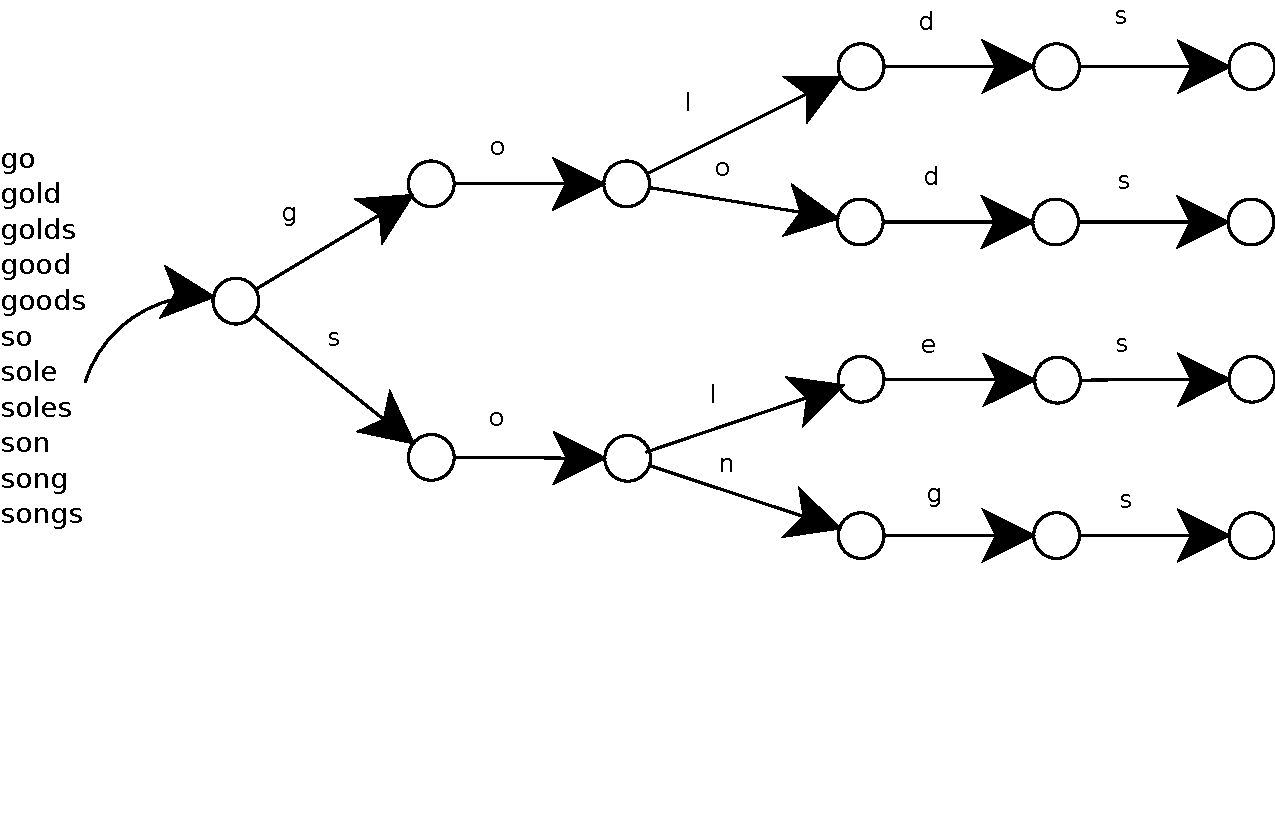
\includegraphics[scale=1]{trie}
\caption{Example of a trie data structure representing a small dictionary consisting of 11 words represented with a trie data structure. End of words is marked with grey nodes.}
\label{fig:trie}
\end{figure}

Appel and Jacobsen showed that the size of the dictionary representation can be reduced with a \emph{Directed Acyclic Word Graph}, referred to as a \emph{DAWG} \cite{fastest}. The DAWG can be constructed by first creating a trie and minimizing it by finding cases where two or more words can share a common letter (node). A new edge is then created from the previous node in one of the words to the other words node. Then the unnecessary edge and node is removed node \ref{fig:dawg}. A trie has a lot of redundancy, because identical edges and nodes is stored, while the DAWG will eliminate duplications. All the identicals is removed, and reduced to only one occurance. In the dawg example fig. \ref{fig:trie} there is 10 nodes and 12 edges. That is significant less than the 17 nodes and 16 edges it consumes in a trie fig. \ref{fig:trie}. Another example is illustrated in \cite{fastest}. A dictionary consisting of more than 100 000 words occupies 0.5 MB with a trie, but is reduced to only 175 kB with a DAWG.

\begin{figure}[h]
\centering
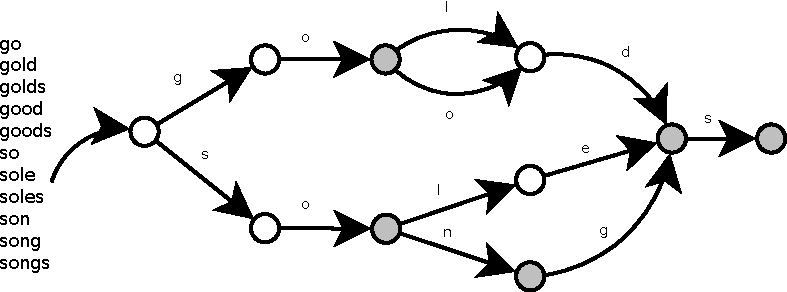
\includegraphics[scale=1]{dawg}
\caption{Example of a small dictionary consisting of 11 words represented with a DAWG. End of words marked with grey nodes.}
\label{fig:dawg}
\end{figure}

\subsection{Word generation algorithm}
Finding and forming words to lay out on the board is difficult. Appel and Jacobsen presented a solution to the problem by reducing the board to one dimension. Instead of searching both up and right at the same time it is possible to generate words only horizontally. The argument is that generating a word vertically is basically the same thing as generating a word horizontally. The only difference is that the board is transposed. Therefore, the word generation algorithm is limited to only find words horizontally. So two searches is done for each move, where one of them with a transposed board. \cite{fastest}


\subsubsection{Anchor squares}
A key in the algorithm implemented are the \emph{anchor squares}, which are the empty squares next to squares occupied by letters as can be seen in the figure \ref{fig:anchors}. These are important since words can only be built from already existing tiles. In the first move of the game there is only one anchor; the center square, since the word in the first turn always has to be placed on top of the center square.

\begin{figure}[h]
\centering
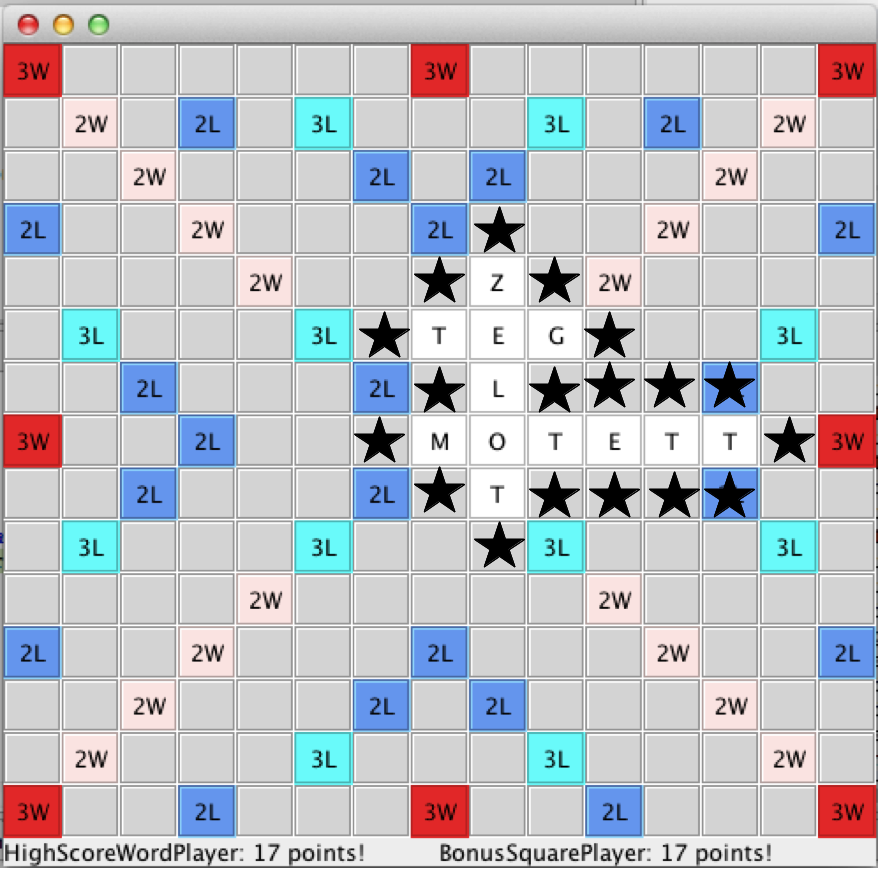
\includegraphics[scale=0.3]{anchors}
\caption{Anchor squares. The adjacent tiles are the anchor tiles from which the word generation begins.}
\label{fig:anchors}
\end{figure}

\subsubsection{Cross-checks}
The set of available legal letters for one square is in Appel and Jacobsen's paper \cite{fastest} referred to as a \emph{cross-check set}. When placing a word horizontally, the vertically placed letters also have to form a legal word. It is quite easy to establish that if a word is placed horizontally, the vertical word can increase with only one letter at a time. This makes it possible to calculate, for each anchor square, which set of letters that are possible to place at that square. The calculations can be made and saved after each move, and allows the algorithm to place a word by row, without considering the rest of the board. 

\subsection{Game strategies}
\label{sec:strategies}
Some of the different Scrabble game strategies is:

\begin{itemize}
\item {\bf Difficult letters}: letters with high score are usually more difficult to place and should be used as soon as possible i.e. z.
\item {\bf Balance on the rack}: it is easy to get stuck with only consonants or only vowels on the rack, keeping a good balance can therefore be a good idea to help construct words in the next turn.
\item {\bf Bonus squares}: hitting the bonus squares will generate a higher score. It is also important to occupty them first to destroy the bonus opportunities for the opponent.
\item {\bf Word extensions}: the ability to identify extensions (i.e. prefixes and suffixes) to words, is a key to being a successful player since such moves can generate very high scores, as the word will use many existing tiles \cite{perfectgame}.
\item {\bf Vocabulary}: there are many short words in the language, and it is rewarding if a player can learn many short word letters because they are easy to lay out.
\end{itemize}





\chapter{Implementation}
The study is based on an implementation of the word generator algorithm that follows the example of Appel and Jacobsen \cite{fastest}, with some small modifications. The words generated by the algorithm is the same with a trie as with a DAWG. Since the aim of the study is to only test game strategies and not optimize disk space (as shown in \ref{dic-rep}), a DAWG seemed like a time consuming project and the choice was made to stay with the trie.

A slight limitation of the game rules and play is made in the implementation to make the study fit into the given time span. The game limitations are described in section \ref{sec:limitations}.

Three different agents were implemented with different strategies to follow and they are all described in section \ref{sec:agents}.

\section{Limitations}
\label{sec:limitations}
Almost all tournament play involve only two players. The tests is therefore run with two agents. There exists a large variation of the game rules. The rules used is a slightly simplified version of the most common rules used by clubs and tournament play worldwide \cite{forbund} \cite{ABSP} \cite{NASPA}.

To limit the work load to fit into the time span, some limitations were made to the game. The players have two options during a turn; either lay a word, or pass the turn and receieve zero points. In other words; the possibility to change tiles if no word can be found is removed. 

The bag is minimized, and do not contain any blank tiles or other special letter tiles. The result is that Q and W can never be used. The allowed tiles can be seen in the list in section \ref{letter+table}. In addition, the game is played with by the agents with a Swedish dictionary, 
Den Stora Svenska Ordlistan\cite{dictionary}.

\section{Agents}
\label{sec:agents}
To see which of the very basic strategies listed in section \ref{sec:strategies} is the most successful one against the others, three agents with different strategies were implemented. They will play against each other in order to generate results for later analyze. This section describes the three different agents implemented, and their strategy in the game. In order to evaluate which strategies are the more rewarding, the agents are each implemented with only \emph{one} strategy. The agents will be referred to as the HSW player, the BS player and the BOR player (see section \ref{sec:terminology}).

\subsection{High Score Word player}
One strategy to follow when playing Scrabble is to exploit the fact that som letters are worth more than others. These letter are less frequent in the Swedish language and therefore more difficult to use. Naturally, one would want to use them as soon as there is an opportunity, to not risk difficult situations later in the game. The HSW player prefers placing words including high score letters. By all legal moves generated, the HSW player will choose the one where the word itself has the highest score. The HSW algorithm is as follows:

\begin{lstlisting}
function ChooseMove(inputMove)
	if score of inputMove.word greater than highestScore
		nextMove <- inputMove;
	end if
end function
\end{lstlisting}

The HSW player saves one move. If a better move is found than the one saved, the new move will overwrite the old one.

\subsection{Bonus Square player}
Sometimes, it can be more rewarding to place a relatively short word than a longer one. This is because of the bonus squares is spread out on the board. They can multiply the value of either one letter, or the entire word placed, and can therefore generate high scores. The second agent strives to place words over bonus squares, to hopefully generate a high score. If there is an opportunity to reach several bonus squares, the most rewarding bonus square is chosen from the following graded list. 3W (three word bonus) being most rewarded and then 2W, 3L (two letter bonus) and last 2L.

\begin{lstlisting}
function ChooseMove(inputMove)
	bonus <- 0;
	for each letter in inputMove.word
		squareBonus <- bonus for letter.square;
		if squareBonus greater than bonus
			bonus <- squareBonus;
		end if 
	end for
	
	if bonus is higher than highestBonus
		nextMove <- inputMove;
		highestBonus <- bonus;
	end if
end function
			
\end{lstlisting}

\subsection{Balance On Rack player}
An important thing to think about when playing Scrabble is to plan for the next move. If a player ends up with only consonants on the rack, the possibility of laying out a word is reduced. The third agent tries to always keep a good balance between vowels and consonants on the rack, to help out form words in the next turn. The agent knows the \emph{ideal ratio} and tries to lay out words so that the words left on the rack returns a ratio as close to the ideal ratio as possible. Tests with different ideal ratios are made.

\begin{lstlisting}

function ChooseMove(inputMove)
	ratio <- number of vowels on rack / 
				number of tiles on rack;

	difference <- abs(ratio - idealRatio);

	if difference is less than ratioDifference
		nextMove <- inputMove;
		ratioDifference <- difference;
	end if
end function
\end{lstlisting}

\chapter{Results}
\label{sec:analysis}
Each of the agents has been tested against the others, to let us evaluate the impact of each strategy. Explanations of the agents can be read about in section \ref{sec:agents}. 

Section \ref{sec:conditions} describes under which conditions the tests were made.

Sections \ref{sec:highBalance}, \ref{sec:balanceBonus} and \ref{sec:bonusHigh} show the results from each run.
 
\section{Test conditions}
\label{sec:conditions}
\subsection{Games}
In one run the agents were set to play 1000 games against each other and to minimize the impact of opening the game in the results, both agents started the game 500 times. Each run were made 10 times, so the total result is based on 10 000 games. It was established that there were no significant changes in the results between running 1000 games, and 10 000 games, and would therefore probably be reduntant to make more tests. 

\subsection{Dictionaries}
Two dictionaries were used in the tests; one consisting of only the normal form of each word and the other consisting of all possible forms of each words, where the latter is a set of 480391 words. The former consists of 83247 words. The rules of Swedish Scrabble do not allow words of all forms, but the english does. Therefore, it seemed interesting to compare how the agents would perform with different conditions. There could be situations where for instance the bonus player has an advantage if conjunctions are allowed, since it strives always after covering the bonus squares. The large dictionary could allow the player to place short extensions to already placed words.

The longest word in the used dictionary is ammoniumdiamintetrakistiocyanatokromat. The shortest possible word to place on board is all two letter words Section \ref{regler}. The number of two letter words is 121. Table \ref{table:dictionary+length}.
\begin{table}[h]
\centering
	\begin{tabular}{l | c | c}
	& Base words & All words \\
	\hline
	Mean & 9.5 & 11.2 \\
	\hline
	Longest & \multicolumn{2}{c}{ammoniumdiamintetrakistiocyanatokromat} \\
	\hline
	Shortest & \multicolumn{2}{c}{121 two letter words} \\ 
	\end{tabular}
\caption{Mean, largest and smallest lengths of legal words in the dictionary.}
\label{table:dictionary+length}
\end{table}

\section{High score words vs Balance}
\label{sec:highBalance}

The results from runs over the large dictionary and the small dictionary do not differ that much, as can be seen in figure \ref{fig:bonusBalanceSmallDict} and figure \ref{fig:bonusBalanceLargeDict}.
The BOR player uses a ratio between vowels and consonants on the rack, and strives to keep the ratio after each move. The wanted number of vowels on hand will be referred to as \emph{vowel ratio}. Several tests were made with the BOR player to see if there is any difference when altering the ratio parameter. The ratio is calculated as the number of vowels left on hand divided into the number of consonants left on hand. Table \ref{tab:bor+hsw} shows the results of the runs made with different ideal number of vowels on hand.

\begin{table}[h]
\centering
    \begin{tabular}{ l | l | l }
   	& BOR & HSW \\
   	\hline
   	Wins & 1 & 9999 \\
	Draws & 0 & 0 \\
	Wins when started playing & 0 & 5009 \\   	
	Mean score & 124 & 420 \\
	Median score & 123 & 415 \\	 	 
	Highest score & 299 & 745 \\
	Lowest score & -16 & -12 \\		
    \end{tabular}
\caption{Result from 10 000 games with vowel ratio 1/8 and words in all inflection forms from the Swedish dictionary (480 391 words).}
\label{table:borhswstats}
\end{table}

\begin{table}[h]
\centering
    \begin{tabular}{ l | l | l }
   	& BOR & HSW \\
   	\hline
   	Wins & 1206 & 8762 \\
	Draws & 32 & 32 \\
	Wins when started playing & 643 & 4431 \\   	
	Mean score & 214 & 309 \\
	Median score & 213 & 307 \\	 	 
	Highest score & 407 & 624 \\
	Lowest score & -9 & -19 \\		
    \end{tabular}
\caption{Result from 10 000 games with vowel ratio 8/8 and words in all inflection forms from the Swedish dictionary (480 391 words).}
\label{table:borhswstats}
\end{table}

The results show that the HSW player is generally more successful playing the game. The BOR player does not take the word score in consideration when playing, but only the ratio, and it it obviously not the most rewarding strategy to follow. An interesting observation is that if the BOR agent tries to keep a ratio of vowels close to 1, i.e all tiles being vowels, there is a significant peak in the number of winning games for the agent. On the other hand, trying to keep one vowel on hand after each round seems to not be as smart, since the agent lost almost 100\% of all games.

\graphicspath{{../results/Plots/}}

\begin{figure}[h]
\centering
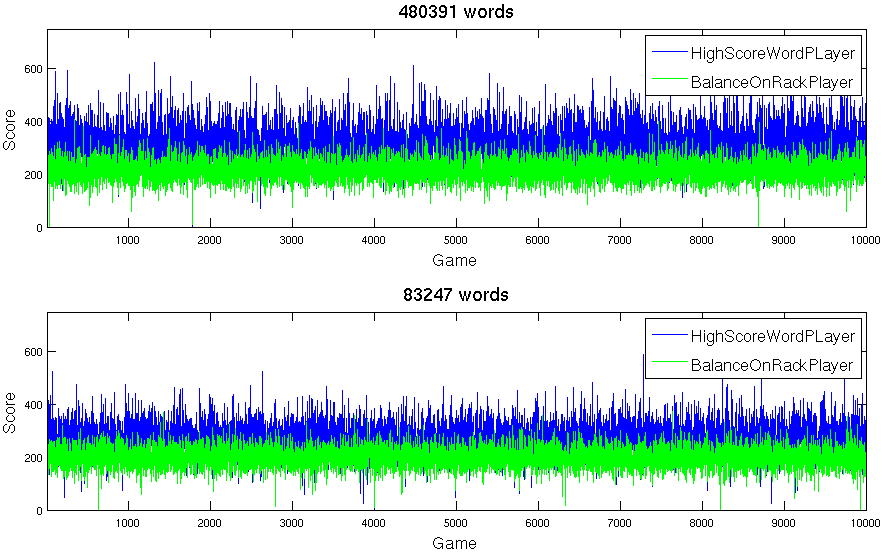
\includegraphics[scale=0.52]{HighBalance8vow_bothDict_cropped}
\caption {Scores with vowel ratio 8/8. Scores of the two players in 1000 games with 83 247 words available.}
\label{fig:bonusBalanceSmallDict}
\end{figure}

\begin{table}[h]
\centering
    \begin{tabular}{ c | c | c p{5cm}}
   	Vowel ratio & HSW wins & BOR wins \\ \hline
	0/8 & 9922 & 73 \\ 
    	1/8 & 9999  & 1 \\ 
    	2/8 & 9484 & 507 \\
    	3/8 & 9777 & 212 \\
	4/8 & 9735 & 262 \\ 
	5/8 & 9627 & 368 \\ 
	6/8 & 9146 & 838 \\ 
	7/8 & 9863 & 134 \\ 
	8/8 & 8762 & 1206 \\
    \end{tabular}
\caption{Winnings over 10000 games depending on vowel ratio. The ratio is defined by the number of vowels divided by the number of tiles on rack.}
\label{tab:bor+hsw}
\end{table}


\section{Balance vs Bonus}
\label{sec:balanceBonus}
The BOR player continues to perform doubtly against the BS player. Also here the BS player consideres what bonus it will be given in a certain move, and chooses the highest one. Naturally the BOR player that only cares about its ratio on the rack will perform worse. The results from runs with different vowel ratio in the BOR player can be seen in table \ref{tab:bor+bs}.

Note that the BOR player is stable with its game results. In figure \ref{fig:bonusBalanceLargeDict} one can see that the BS player in some games made an extremely poor performance, receiving zero points or less, while the BOR player keeps the graph quite thin, i.e. the results differ less from game to game.

\begin{table}[h]
\centering
    \begin{tabular}{ c | c | c  p{5cm}}
   	Vowel ratio & BS wins & BOR wins \\ \hline
	0/8 & 9925 & 72 \\ 
    	1/8 & 9987 & 12 \\ 
    	2/8 & 9670 & 325 \\ 
    	3/8 & 9829 & 165 \\ 
	4/8 & 9818 & 172 \\ 
	5/8 & 9731 & 261 \\ 
	6/8 & 9370 & 620 \\ 
	7/8 & 9859 & 141 \\ 
	8/8 & 9074 & 915 \\ 
    \end{tabular}
\caption{Winnings over 10000 games depending on vowel ratio. The ratio is defined by the number of vowels divided by the number of tiles on rack.}
\label{tab:bor+bs}
\end{table}

\begin{figure}[h]
\centering
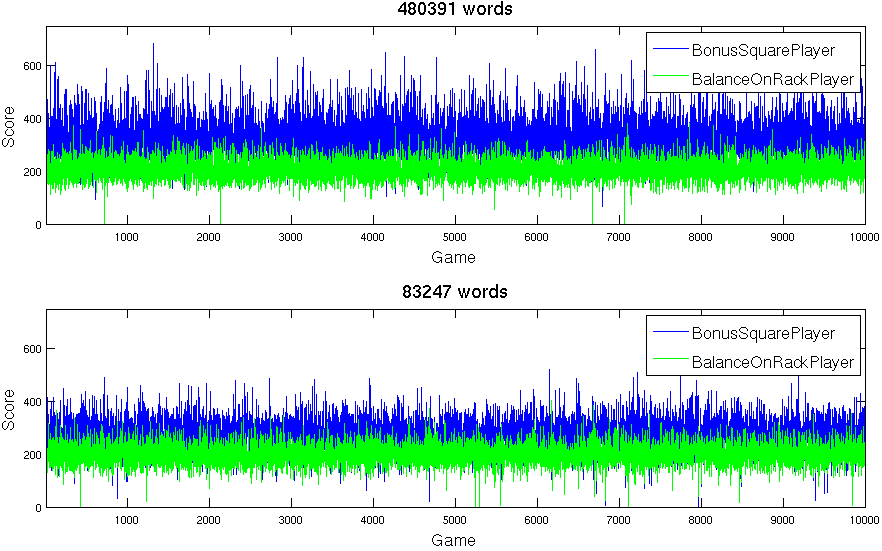
\includegraphics[scale=0.52]{BonusBalance8vow_bothDict_cropped}
\caption {Scores with vowel ratio 8/8. Scores of the two players in 1000 games with 480 391 words available.}
\label{fig:bonusBalanceLargeDict}
\end{figure}



\section{Bonus vs High score words}
\label{sec:bonusHigh}
\emph{BS} wins just over 6 of 10 times against \emph{HSW} when using all inflection forms from the Swedish dictionary table \ref{table:bs+hsw+allwords} and well over 5 of 10 times when only the base forms of words is used table \ref{table:bs+hsw+baseforms}. When \emph{BS} started playing it won 52\% of its wins when using all inflection forms. For \emph{HSW} 53\% of its wins. When using only the base form both of them were winning 51\% its wins when started laying out words.

\begin{table}[h]
\centering
    \begin{tabular}{ l | c | c }
   	& Bonus Squares & High score words \\
   	\hline
   	Wins & 6104 & 3857 \\
   	Draws & 39 & 39 \\   	
	Wins when started playing & 3148 & 2040 \\   	
	Mean score & 308 & 278 \\
	Median score & 301 & 273 \\	 	 
	Highest score & 724 & 606 \\
	Lowest score & 85 & 61 \\		
    \end{tabular}
\caption{Result from 10 000 games with words in all inflection forms from the Swedish dictionary (480 391 words).}
\label{table:bs+hsw+allwords}
\end{table}

\begin{table}[h]
\centering
    \begin{tabular}{ l | c | c }
   	& Bonus Squares & High score words \\
   	\hline
   	Wins & 5427 & 4521 \\
   	Draws & 52 & 52 \\
	Wins when started playing & 2758 & 2314 \\   	
	Mean score & 248 & 240 \\
	Median score & 246 & 234 \\	 	 
	Highest score & 488 & 506 \\
	Lowest score & -15 & -11 \\		
    \end{tabular}
\caption{Result from 10 000 games with only words in base form from the Swedish dictionary (83 247 words).}
\label{table:bs+hsw+baseforms}
\end{table}

The resulting mean, median, highest and lowest scores is significant higher when using all inflection forms. Lowest score is negative for both players when using only base forms. \emph{BS} mean score is 24\% higher in table \ref{table:bs+hsw+allwords} compared to table \ref{table:bs+hsw+baseforms}. The same applies for the end score which is higher when using all words Appendix Figure \ref{fig:bs+hsw+totalscores}.

\begin{figure}[h]
\centering
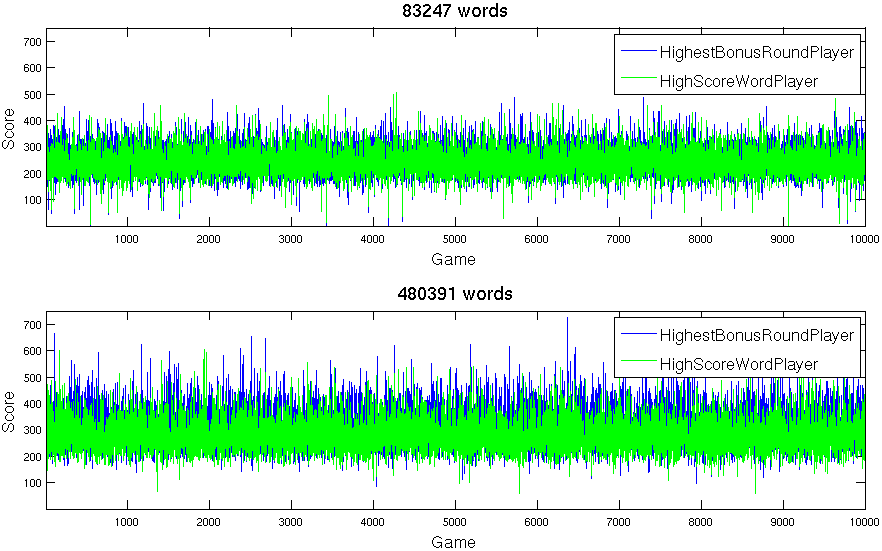
\includegraphics[scale=0.52]{Highest_Bonus_Round_vs_High_Score_Word_10000_cropped}
\caption {End scores of the two players in 10000 games. Upper graph with base words only and lower graph with all inflection forms.}
\label{fig:bs+hsw+totalscores}
\end{figure}



\chapter{Conclusions}
\section{Discussions}
\subsubsection{BOR player}
The BOR player is significantly better with a vowel ratio of 8/8. It can probably be explained from the fact that when choosing a move, and the vowel ratio is 8/8 (1) it is easier for the agent to place longer words. Imagine the agent placing a word using all tiles but one, and the remaining tile on hand is a vowel. This would be a preferable move if the ratio is 1, but not if the ratio is less. If the ratio would be 4/8 for example, the agent would choose a move that leaves two tiles, where one is a vowel, over the move with a longer word. 

\subsubsection{HSW player}
High score word player conclusions go here.

\subsubsection{BS player}
Choosing to place words that will occupy a bonus square is rewarding. It will not only give a high score but will also destroy the possiblity for the opponent to reach a bonus square.

It has active playing style with the mission to conquer the bonus squares at all cost. With the power of a big dictionary it will have a higher probability to reach a bonus. It is easy to extend words already on board when having the possibility to use all inflection forms of words. The end score will also be higher Figure \ref{fig:bs+hsw+totalscores}. When using only base words it will struggle to find bonus squares. This is due to 

\section{Conclusions}
TODO kanske använda denna An agent who calculates the total score of a move and chooses the highest one will easily win over the tested agents in this study. 


\begin{thebibliography}{100}  
  \bibitem{perfectgame} Sheppard, B., 2002, Towards Perfect Play of Scrabble, Maastricht.
  \bibitem{fastest} Appel A. W., Jacobson, G. J., 1985, The World’s Fastest Scrabble Program, Commun. ACM, 31(5), 572-585, May 1988.
\bibitem{faster} Gordon, S. A., 1993, A Faster Scrabble Move Generation Algorithm, Software - Practice and experience, Vol. 24(2), 219-232, February 1994.
\bibitem{ai} Russell S., Norvig P. Artificial Intelligence: A Modern Approach 3rd ed. Prentice Hall. 2009
\bibitem{inforetrieve} Manning C. D., Raghavan P., Schütze H., Introduction to Information Retrieval, Cambridge University Press, 2008, p. 49-65.
\bibitem{dictionary} Den stora svenska ordlistan (Swedish dictionary), http://code.google.com/p/dsso/downloads/detail?name=dsso-1.52.txt\&can=1\&q=
\bibitem{forbund} Swedish tournament rules by Svenska Scrabbleförbundets, http://www.scrabbleforbundet.se/index.php?option=content\&task=view\&id=16\&Itemid=39
\bibitem{ABSP} World English-Language Scrabble Players’ Association (WESPA) rules, http://www.wespa.org/rules/RulesV2nov11.pdf
\bibitem{NASPA} North American SCRABBLE Players Association official tournament rules, http://www.scrabbleplayers.org/wiki/images/a/af/Rules-20110605.pdf
\end{thebibliography}
\end{document}